\documentclass{article}

\usepackage[letterpaper, margin=0.6in, bottom=1in]{geometry}
\usepackage{amsmath, amsfonts, amsthm, amssymb}
\usepackage{setspace}
\usepackage{enumitem}
\usepackage{mdframed}
\usepackage[colorlinks]{hyperref}
\usepackage{graphicx}
\usepackage{calc}
\usepackage{mlmodern}
\usepackage{soul}

\title{\vspace*{-40pt} Expository Materials on Solids and Surfaces of Revolution}
\author{Jayden Li}
\date{AP Calculus BC 2024-25}

\begin{document}
\setstretch{1.25}
\fontsize{11pt}{12pt}\selectfont
\setlength{\abovedisplayskip}{\abovedisplayskip/2}
\setlength{\belowdisplayskip}{\belowdisplayskip/2}
\setlength{\parindent}{0pt}
\setlength{\parskip}{2ex plus 0.5ex minus 0.2ex}
\maketitle

\begin{abstract}
	We create a series of animations using the Manim library to visualize and derive the formulas for the area of a surface of revolution and the volume of a solid of revolution, specifically disc integration and cylindrical shells. We then create a guided problem set showing students how to apply said formulas to a real-world problem.
\end{abstract}

\section{Introduction}

As an AP Calculus BC student, one of the most difficult units was on solids of revolution. While not as complicated as some other topics, it was definitely hard to visualize. Our graphing calculators (that we use, anyway), whiteboards and papers all exist in $\mathbb R^2$, while revolutions require us to visualize objects in three dimensions.

I drew heavy inspiration from Grant Sanderson's \href{https://www.youtube.com/c/3blue1brown}{3blue1brown} YouTube channel. I used his style and animation library to create these animations, and while there was learning involved, making videos with these tools was a lot easier than expected.

I hope to step through the derivation, which are included in the notes of problem sets, through visual demonstration. This will include rotating around the object and showing what a Riemann sum looks like in three dimensions.

All Manim animations are written as Python scripts. The source code for all animations can be found in my GitHub repository at \url{https://github.com/glolichen/calc-bc-project}. Final videos are available on my YouTube channel.
\begin{itemize}[topsep=0pt]
	\item Disc method: \url{https://www.youtube.com/watch?v=yVkQnoRSHuQ}
	\item Area of a surface of revoution: \url{https://www.youtube.com/watch?v=AMNdfO6yOB4}
\end{itemize}

The rest of this documents is a guided exercise for calculating volumes of revolution.

\section{Acknowledgements}

I would like to thank the creators and maintainers of \href{https://www.manim.community/}{Manim Community Edition} and its documentation. Clearly, my project is impossible without their dedication to the Manim library.

It is clear my project has significant stylistic similarities to 3blue1brown, whose videos have inspired be significantly and made me see the power and beauty of visualization and visual derivations.

\newpage

\begin{center}
	\textbf{\underline{A Gift for Mrs. Montgomery}}

	AP Calculus BC, 2025-26
\end{center}

Jayden Li\footnote{I received permission from Jayden Li to use his likeness.}, Peddie Class of 2026, has a CYU in AP Calculus BC tomorrow. His GPA is currently an abysmal 2.54\footnote{His grades are kinda \textit{cheesy}, becuase AP US History made it go \textit{poof}.} and he knows he will be cooked by the upcoming CYU, which is on Taylor Series. He hears this CYU is the most difficult in the course, including from Mrs. Montgomery herself.

Failing the CYU is not an option. Not only will Jayden Li's mother be extremely angry, he will probably also receive an Academic Warning\footnote{See page 10 of the 2024-25 Peddie School Student and Family Handbook.}! All because of an extremely difficult CYU on Taylor Series.

Fortunately, Allison Li\footnote{I received permission from Allison Li to use her likeness.}, Peddie Class of 2027, has proposed an easy solution for Jayden. It turns out Mrs. Montgomery has an insatiable love for vases, which she uses to store flowers in her house. Since Mrs. Montgomery also loves math and equations, Allison thinks she has the perfect gift for Mrs. Montgomery ahead of the CYU. They hope the gift will bring happiness to Mrs. Montgomery, resulting in a less difficult CYU with fewer strange functions and questions.

Tiffany Tian\footnote{I received permission from Tiffany Tian to use her likeness.}, Peddie Class of 2027, also wants to make sure Jayden does not receive a meeting with Mr. Wriede, and agrees to turn\footnote{``To shape (something) symmetrically by rotating it against a stationary cutting tool, as on a lathe.'' (Wiktionary)} the vase on a lathe in the Izzo Design Laboratory.

Looking from the side, the cross sectional shape of the vase can be modeled by the function $f(y)=\cos(y-1)+2$. \textbf{\st{Cutting} Turning the vase on the lathe has the same effect as revolving the function $f(y)$ around the $y$-axis.} The units of $f$ (and the vase) are in meters. The vase is of height $6$ meters, and its base is at $y=0$. 


\begin{itemize}
	\item[(a)] Mrs. Montgomery is not sure how happy she should feel about the vase. There has recently been a flood in Hightstown and she wants to store at least $80$ cubic meters of flood water in the vase. Is this possible?


	\item[(b)] Mrs. Montgomery is concerned the vase may be too heavy to carry, and the vase's mass is directly proportional to its surface area. Please calculate the surface area of the vase for Mrs. Montgomery to decide whether she can safely move it. You may use a graphing calculator.
\end{itemize}

\newpage

\begin{equation*}
	f(y)=\cos(y-1)+2
\end{equation*}
\setstretch{2}
\begin{itemize}[topsep=0pt]
\item[(a)]
	\begin{enumerate}
		\item First, we are revolving $f(y)$ around the $y$-axis. Since the function $f$ is in terms of $y$, we integrate along the \underline{\hspace{0.5in}} axis (with respect to \underline{\hspace{0.5in}}), which is parallel to the axis of rotation. Consider the cross section of the vase along the axis of integration. This means we can use \underline{(disc / washer / cylindrical shells)}.

		\item The base of the vase is at $y=\underline{\hspace{0.5in}}$, and since the vase's height is $6$ meters, the top of the vase is at $y=\underline{\hspace{0.5in}}$. The limits of integration is $[\underline{\hspace{0.5in}}, \underline{\hspace{0.5in}}]$.

		\item The radius of each disc is \underline{\hspace{2in}}.

		\item Recall the disc method formula: $\displaystyle V=\pi \int_{a}^{b}(\text{Radius})^2\,\mathrm{d}y$. As an integral, the volume of the solid is:
			\vspace{1in}

		\item Evaluate the integral below. \textbf{The vase should store more than $80$ cubic meters of water.}
	\end{enumerate}
	\newpage
	
\item[(b)]
	\begin{enumerate}
		\item Let's consider the surface area of the vase as a Riemann sum. Let there be $n$ subdivisions, each of height $\Delta y$. Each subdivision is a \textbf{truncated cone}:
		\begin{center}
			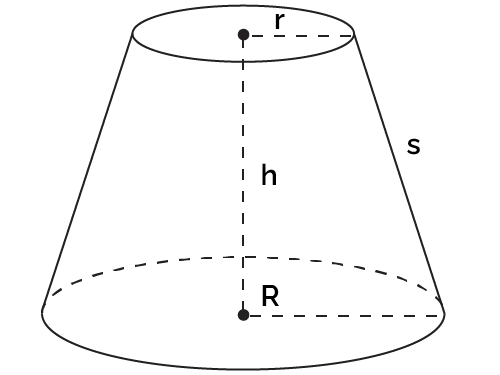
\includegraphics[height=1.7in]{TruncatedCone.png}

			\url{https://www.omnicalculator.com/math/truncated-cone}
		\end{center}

	\item Let's consider the $i$th subdivision. We call the bottom $y$-value $y_i$, and the top $y_{i+1}$. In the above picture, we would have $r=\underline{\hspace{1in}}$ and $R=\underline{\hspace{1in}}$ (hint: the radius $r$ and $R$ is the distance between the $y$-axis and the function $f(y)$).

	\item The height of the truncated cone is $y_{i+1}-y{i}=\underline{\hspace{1in}}$.

	\item We need to calculate the surface area of the truncated cone, excluding the top and bottom faces. This is because in the Riemann sum, the top and bottom faces are directly against another subdivision and do not count towards the area of the surface of revolution. This is exactly the area of the slant, which is $\pi s(R+r)$.

	\item We know $R$ and $r$, but need to find $s$. Notice we can construct a right triangle with $s$ as the hypotenuse. One of the legs is the height of the truncated cone: $\underline{\hspace{1in}}$.

	\item The other leg is: $\underline{\hspace{1in}}-\underline{\hspace{1in}}=\underline{\hspace{2in}}$.

	\vspace{0.25in}
	\item By the Pythagorean theorem, $s$ equals \hrulefill

	\item Using the formula $\text{Slant area}=\pi s(R+r)$, write down the area of the slant below.
		\vspace{0.8in}
		\begin{mdframed}
			You should have $\displaystyle \pi \sqrt{\left( \Delta y \right)^2+\left( f(y_{i+1})-f(y_i) \right)^2}\left( f(y_i)+f(y_{i+1}) \right)$, or something equivalent.
		\end{mdframed}

	\item Now write down the sum of the slant areas of $n$ subdivisions, as $n$ approaches infinity.
		\vspace{-0.2in}
		\begin{equation*}
			SA
			=\lim_{n\to\infty}\sum_{i=1}^{n}\hspace{5in}
		\end{equation*}

	\item See if you can factor out the $(\Delta y)^2$ from the square root. The root should read $\displaystyle \sqrt{1+\frac{\phantom{(f(y_{i+1})-f(y_1))^2}}{(\Delta y)^2}}$. Also, $y_{i+1}=y_i+\underline{\hspace{1in}}$. Make this substitution in the two appearances of $y_{i+1}$.
		\vspace{1in}

	\item As $n\to\infty$, $\Delta y\to \underline{\hspace{1in}}$. So $y_{i+1}=y_i+\Delta y\to \underline{\hspace{1in}}$. In which of the two appearances of $f(y_i+\Delta y)$ in the above equation can we actually make this substitution? (hint: notice $(\Delta y)^2$ in the denominator, and remember the limit definition of the derivative)
		\vspace{1in}
		\begin{mdframed}
			You should have $\displaystyle \lim_{n\to\infty}\sum_{i=1}^{n}\pi \Delta y \sqrt{1+\frac{\left( f(y_i+\Delta y)-f(y_i) \right)^2}{(\Delta y)^2}}\left( f(y_i)+f(y_i) \right)$, or something similar.
		\end{mdframed}

		\vspace{0.125in}
	\item By the limit definition, $\displaystyle f'(y_i)=\lim_{\Delta y\to0}\frac{\hspace{2in}}{\hspace{2in}}$. 
		\vspace{0.125in}

	Do you see this in your answer to 11? If yes, rewrite it in terms of $f'(y_i)$. Make any trivial simplifications.
		\vspace{1in}

		\begin{mdframed}
			You should have $\displaystyle \lim_{n\to\infty}\sum_{i=1}^{n}2\pi f(y_i) \Delta y \sqrt{1+(f'(y))^2}$, or something similar.
		\end{mdframed}
	
		\item Is this in the form of a Riemann sum? Write the above sum as an integral, and evaluate it by calculator.
	\end{enumerate}
\end{itemize}


\newpage
\setstretch{1.25}

\begin{center}
	\textbf{\underline{A Day at the Blair Academy}}

	\st{AP Calculus BC} Calculus, 2025-26\footnote{Apparently, the Blair Academy does not offer AP courses.}
\end{center}

After a winter term trapped inside the robotics lab, Jayden Li wants to connect with nature more. To do so, he has enrolled at the Blair Academy for the spring term.

After a humiliating defeat at the hands of the Peddie School at the 2024 ``Peddie Day'' event, the students of Blair are finding innovative ways to win the 2025 ``Peddie Day,'' where they seek to snatch the ``Potter-Kelly Cup'' from its rightful owners.

They discussed many ways to do so. Someone proposed to simply win more matches at ``Peddie Day,'' but this idea was dismissed as ``unrealistic.'' Instead, they are attempting to find innovative devices and techniques to distract Peddie atheletes, allowing the Blair Academy to snatch the win right under Peddie's noses.

They have come up with the following object to use as a Vuvuzela\footnote{\url{https://www.youtube.com/watch?v=0XViRxTv0kc}}. This is known as a \textit{Gabriel's Horn}, and is obtained by revolving the function $f(x)=1/x$ on the interval $[1,\infty)$ around the $x$-axis.

\begin{center}
	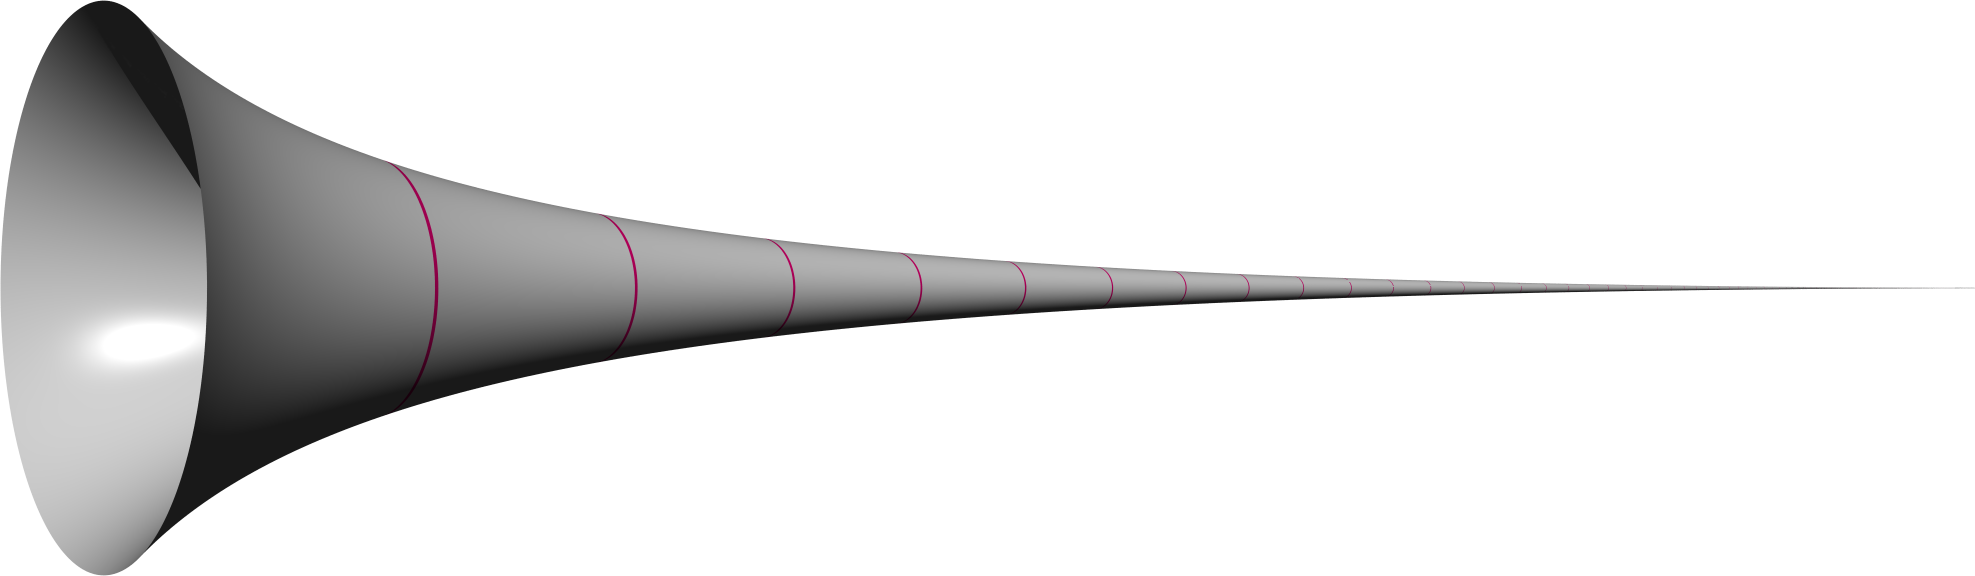
\includegraphics[width=0.8\linewidth]{GabrielHorn.png}
	\url{https://en.wikipedia.org/wiki/Gabriel%27s_horn}
\end{center}

\begin{itemize}[topsep=0pt]
	\item[(a)] The Blair Academy's version of Mr. Tackett wants to know how much material the ungraciously-unprofessional object will use (which equals its surface area).
	\item[(b)] What is the volume of the Vuvuzela?
	\item[(c)] Before they can use this object at the 2025 ``Peddie Day,'' they must paint the device in navy blue. Is this possible? Why or why not?
\end{itemize}

Jayden's classmates at the Blair Academy are unable to answer the above questions, despite being seniors who will graduate in a few weeks. Save the day by solving it for them!\footnote{Inspired by \url{https://www.reddit.com/r/UofT/comments/1ijkea6/uwaterloo_math_138_question_yall_are_dumb_asl_lmao/}}

Note: these problems include \textit{improper integrals} in the form $\displaystyle \int_{a}^{\infty}f(x)\,\mathrm{d}x$. If $F$ is the antiderivative of $f$, then:
\begin{equation*}
    \int_{a}^{\infty}f(x)\,\mathrm{d}x
	=\lim_{t\to\infty}\int_{a}^{t}f(x)\,\mathrm{d}x
	=\lim_{t\to\infty}\left[F(x)\right]_{a}^{t}
	=\lim_{t\to\infty}F(t)-F(a)
\end{equation*}

If $\lim_{t\to\infty}F(t)$ diverges, then the integral also diverges.

\end{document}


